\section{Технический проект}
\subsection{Общая характеристика организации решения задачи}
Необходимо спроектировать и разработать веб-мессенджер в ретро-стиле для обмена текстовыми сообщениями между пользователями. Все пользователи общаются в общем групповом чате, и нет личных контактов. Серверная часть реализована на языке программирования Python с использованием SQLite 3 для хранения сообщений и информации о пользователях. Веб-клиент реализован с использованием HTML, CSS и JavaScript.

\subsection{Описание используемых библеотек и языков программирования}
Проект реализован с использованием следующих языков программирования и технологий:

\subsubsection{Серверная часть: Python}
Python используется для реализации серверной части мессенджера. Он обеспечивает взаимодействие с базой данных SQLite 3, обработку запросов от клиентов, отправку и прием сообщений.

\subsubsection{Веб-клиент: HTML, CSS, JavaScript}
Для создания веб-клиента используются технологии веб-разработки. HTML используется для структуры веб-страницы, CSS - для стилей и внешнего вида, JavaScript - для взаимодействия с сервером, обновления данных на странице и реализации интерактивности.

\subsubsection{База данных: SQLite 3}
SQLite 3 используется для хранения сообщений и информации о пользователях. Это легковесная база данных, которая интегрируется в проект и обеспечивает эффективное хранение и извлечение данных.

\subsection{Основные функции мессенджера}
Проект реализует следующие основные функции мессенджера:

\begin{itemize}
	\item Отправка сообщений: Пользователи могут отправлять текстовые сообщения в общий групповой чат.
	\item Отображение сообщений: Веб-интерфейс отображает сообщения, отправленные всеми пользователями, с указанием отправителя.
	\item Обновление сообщений в реальном времени: Новые сообщения отображаются на веб-странице без необходимости перезагрузки.
	\item Хранение сообщений и информации о пользователях: Сервер хранит сообщения и информацию о зарегистрированных пользователях в базе данных SQLite 3.

\end{itemize}

\subsection{Технические детали проекта}
\subsubsection{Обновление сообщений в реальном времени}
Для обновления сообщений в реальном времени используется технология WebSocket. Когда пользователь отправляет новое сообщение, сервер немедленно уведомляет всех подключенных пользователей о появлении нового сообщения, и их веб-страницы обновляются динамически.

\subsubsection{Авторизация пользователей}
Для обеспечения безопасности и отделения пользователей мессенджера, каждый пользователь проходит процедуру авторизации. Пользователь вводит свое имя при запуске мессенджера, и это имя используется как его идентификатор при отправке сообщений и взаимодействии с сервером.

\subsubsection{Хранение данных}
Информация о пользователях и сообщения хранятся в базе данных SQLite 3. Каждое сообщение содержит информацию об отправителе, тексте сообщения и времени отправки. Таблица пользователей содержит уникальные имена пользователей и их идентификаторы.

\subsubsection{Интерфейс веб-клиента}
Интерфейс веб-клиента состоит из области отображения сообщений и формы для отправки новых сообщений. Сообщения отображаются в хронологическом порядке с указанием имени отправителя и времени отправки. Форма отправки нового сообщения включает поле ввода текста и кнопку для отправки.


\subsection{Структура проекта}
\subsubsection{Структура серверной части}
Структура серверной части мессенджера представлена следующим образом:

\begin{figure}[H]
	\centering
	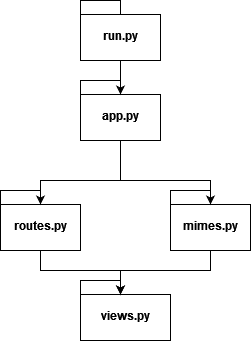
\includegraphics[width=0.7\linewidth]{images/Server_diag}
	\caption{Диаграмма компонентов сервера}
	\label{fig:serverdiag}
\end{figure}

\subsubsection{Структура веб-клиента}
Структура веб-клиента мессенджера представлена следующим образом:

\begin{figure}[H]
	\centering
	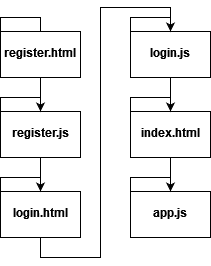
\includegraphics[width=0.7\linewidth]{images/klient_diag}
	\caption{Диаграмма компонентов веб-клиента}
	\label{fig:klientdiag}
\end{figure}

\subsubsection{Диаграмма классов}
На рисунке \ref{fig:classdiag} изображена диаграмма классов для моего проекта веб-мессенджера. Данная диаграмма визуализирует взаимодействие между различными классами, представляющими пользователей, сообщения, чаты, элементы управления и другие основные компоненты системы.


\begin{figure}
	\centering
	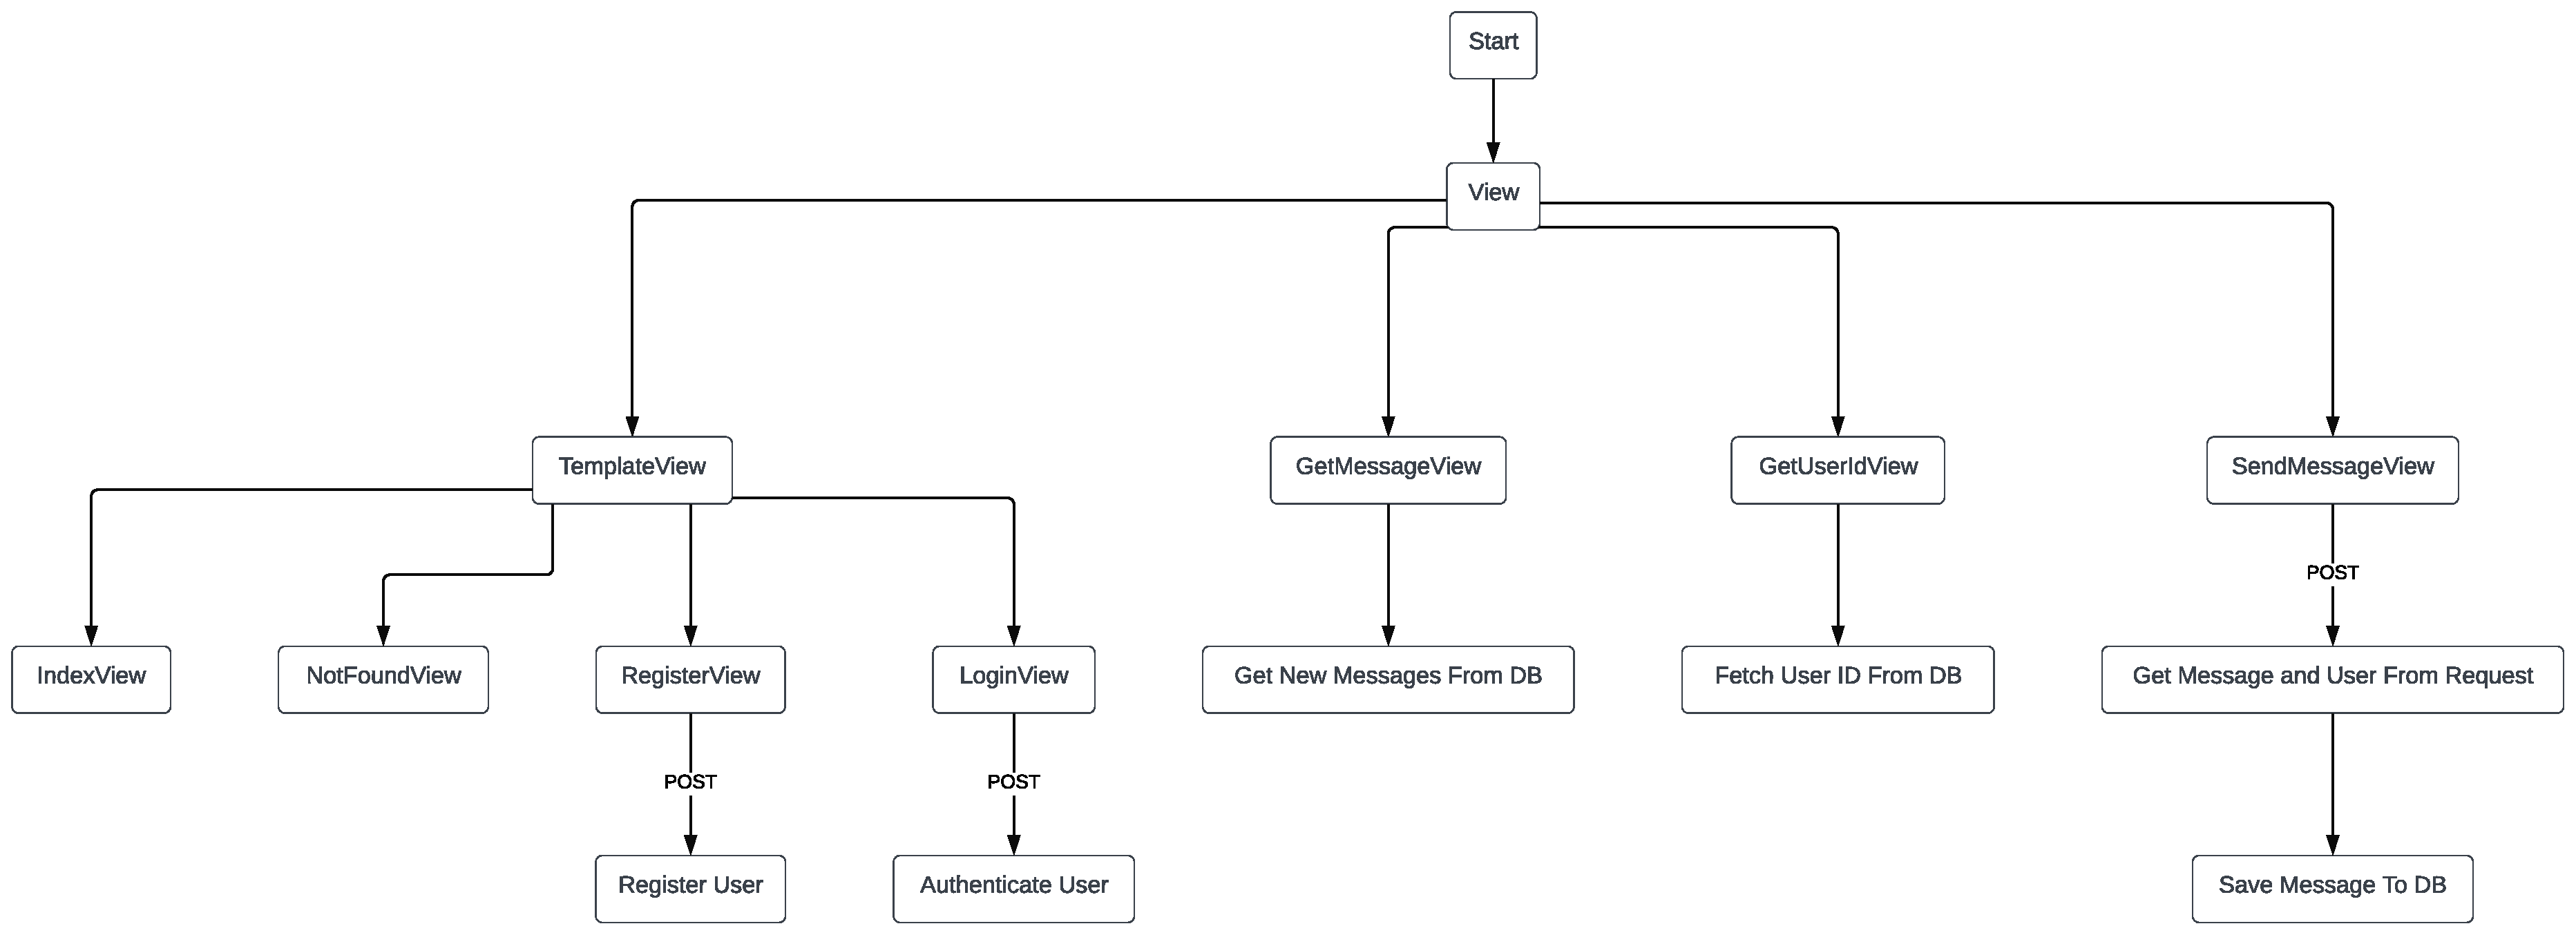
\includegraphics[width=0.7\linewidth]{images/class_diag}
	\caption{Диаграмма классов}
	\label{fig:classdiag}
\end{figure}


